\documentclass[12pt]{article}
\usepackage{amsfonts, epsfig}
\usepackage[authoryear]{natbib}
\usepackage{graphicx}
\usepackage{fancyhdr}
\pagestyle{fancy}
\lfoot{\texttt{comsm0094.github.io}} \lhead{LC\&B - 01.4 areas of the cortex - Conor} \rhead{\thepage} \cfoot{}
\begin{document}

\section*{Parts of the brain - the cortex}

The brain has different parts, different areas made up of different
types of neurons arranged in different structures. This might not be
so obvious looking at stardard pictures of the brain, like the one in
Fig.~\ref{fig_brain}, you are mostly looking at the cortex, which
forms the outer surface of the mammalian brain. Even the cortex,
however, has different areas, as we will discuss in this section.

\begin{figure}[tbhp]
  \begin{center}
  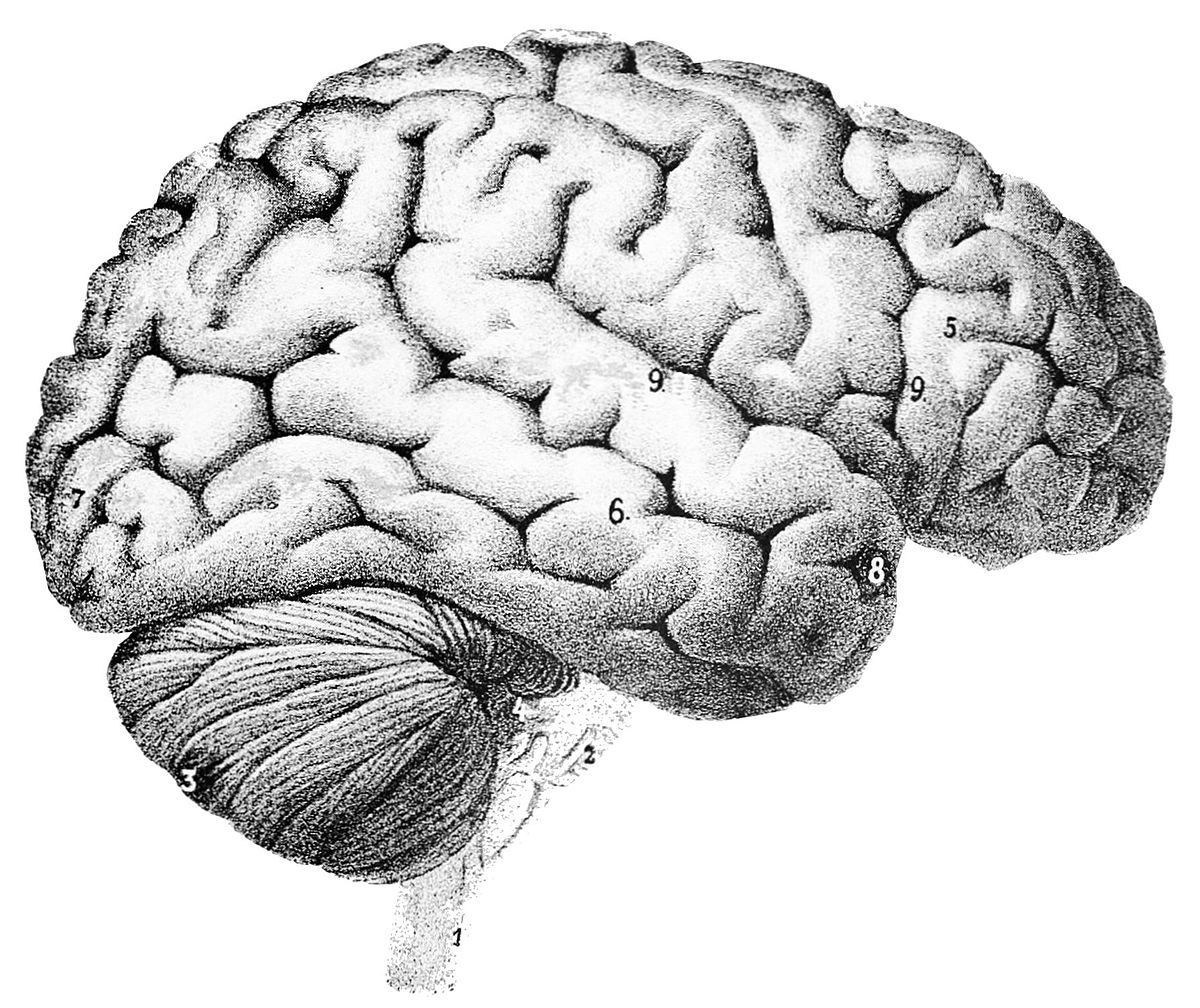
\includegraphics[width=6cm]{brain.jpg}
\end{center}
  \caption{\textbf{A picture of the brain}; when we look at a human
    brain we mostly see cortex, though in this case we can also see
    the cerebellum, labelled 3. Figure from
    \texttt{wikipedia}\label{fig_brain}}
\end{figure}

The different parts of the brain have different functions, but we
don't think any of these functions is `thinking'; that is the function
of the whole brain, the product of the cooperative action of all the
diverse brain regions. Here we will have a quick tour of different
brain parts, their structure and their function; some of these regions
we will revisit in more detail, others not, but the main point here is
to give a feeling for the variety across regions of the brain and the
types of specialization they exhibit, in their function and in how
they perform it. This account will be somewhat mammal, or even human,
focussed.

\subsection*{The cortex}

The cortex, or more specifically the \textsl{cerebral cortex} forms
the outer layer of the mammalian brain. In the human brain it contains
14-15 billion neurons and the extent of the cortex is one of the
distinctive feature of the human brain, Fig.~\ref{fig_cortex}. 

\begin{figure}[tbhp]
  \begin{center}
  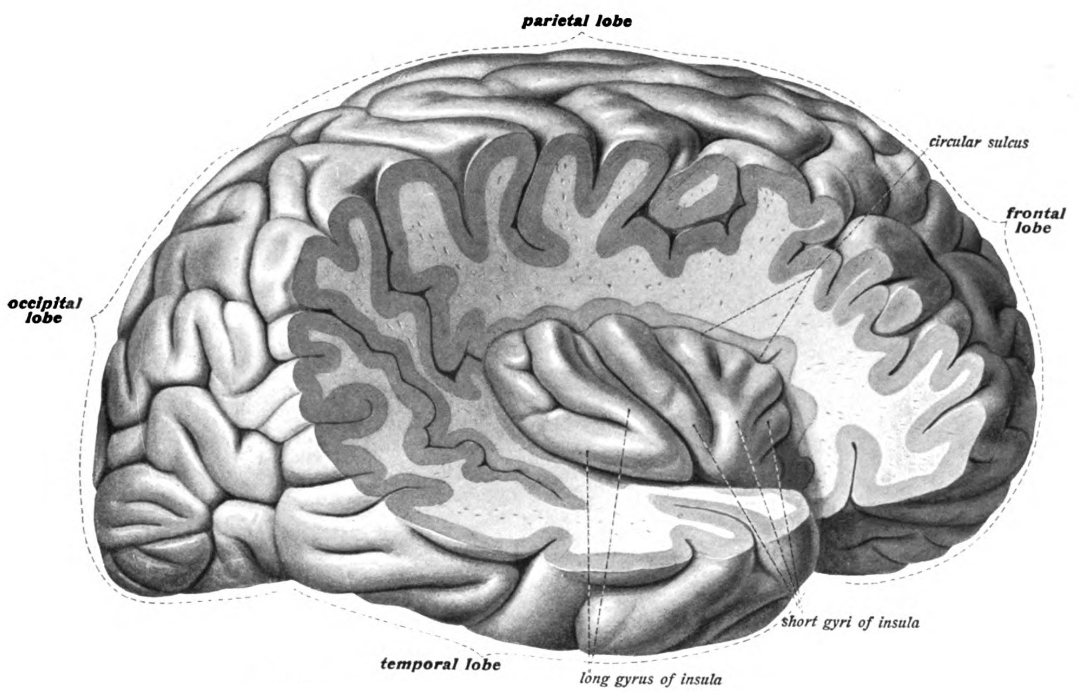
\includegraphics[width=6cm]{cortex.png}
\end{center}
  \caption{\textbf{The cortex}; the cortex, in grey in this picture,
    is an outer layer; in primate brains, and particularily in human
    brains, the cortex has become very folded in an effort to fit more
    in, space is short because we need a lot of cortex to be smart,
    and our heads are smallish because of contraints on human anatomy
    related to standing upright limit the size of head that a baby can
    have at birth. The grooves are called sulci, the ridges are gyri. Figure from \texttt{wikipedia}\label{fig_cortex}}
\end{figure}

The cortex is thin, two to five milimetres thick in humans and
arranged in layers. Most of the cortex has six layers, Fig.~\ref{fig_layers}, distinguished by
different types of neurons and different connectivity
patterns. Connectivity isn't homogenous either, across the surface of
the cortex it is divided into columns, with cells inside a given column having many of the connections within the column.


\begin{figure}[tbhp]
  \begin{center}
  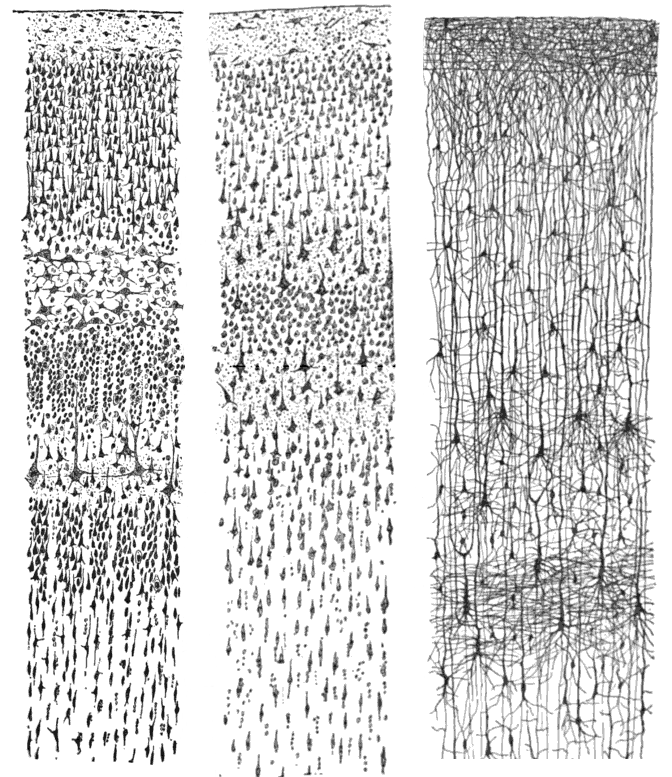
\includegraphics[width=6cm]{layers.png}
\end{center}
  \caption{\textbf{Layers of the cortex}; in these illustrations by
    Cajal we see different cortical layers, the middle and left how
    soma and the right the dendrites; when Cajal did his drawing he
    would stain the cells to make some visible, only a random subset
    take up the stain, otherwise they couldn't be easily distinguished
    by microscope and different staining chemicals showed different
    parts of the neuron. The left is visual cortex, the middle is
    motor cortex. The middle panel shows motor cortex and the Figure
    from \texttt{wikipedia}\label{fig_layers}}
\end{figure}




\subsection*{Broca's area}

Broca's area is perhaps not the obvious place to start when discussing
brain regions, it is an area of the cortex responsible for some
aspects of speech. However, it does make sense to discuss it because
of its historical status in the history of our understanding of how
different part of the brain are specialized to different functions.

Alot of our early understanding of the brain came from studying
patients with brain lesions; modern neuroscience often seems very
focussed on animal studies and this has allowed us to make progress in
understanding the brain in a precis way, but information from patients
still helps guide our subject by linking brain function to our
experiences and abilities.

Louis Victor Leborgne was a patient of the nineteenth century
neurologist Pierre Paul Broca; he is usually known by the name `Tan'
because at 30 that was the only word he could say. Interestingly,
Leborgne could understand language and could express understanding and
emotion with the intonation of how he said `Tan', that was the only
word he could produce.

There are two well-known fictional characters based on Leborgne, Garp,
from John Irving's novel of the same name, who differs from Leborgne
in his ability to understand speech and Hodor from \textsl{The Game of
  Thrones}, particularly in the HBO TV series; although Hodor's
limited speech was ultimately attributed to nonsense magical events,
he shows precisely the behaviour described above, he could understand
speech and express emotion though intonation, but could not say any
word but `Hodor'.

Sadly Leborgne died, in 1861, soon after he was visited by Broca; an
autopsy reveals that he had a very specific lesion in his brain caused
by syphilis; a picture is shown in Fig.~\ref{fig_broca}. This lead
Broca to suggest that this area was responsible for the production of
speech and that lesions to this part of the brain cause
\textsl{expressive aphasia}, aphasia means a problem with speech and
in expressive aphasia the problem is with the production of
speech. This was confirmed by subsequent patient, including another
studied by Broca, Lelong, who only had five words. Another part of the
brain, Wernicke's area, was soon identified with \textsl{fluent
  aphasia}, an inability to understand speech while retaining access
to words. A patient with fluent aphasia can have a large vocabulary
but produces what is called `word salad', lots of words included many
which are not related to the subject of speech.

\begin{figure}[tbhp]
  \begin{center}
  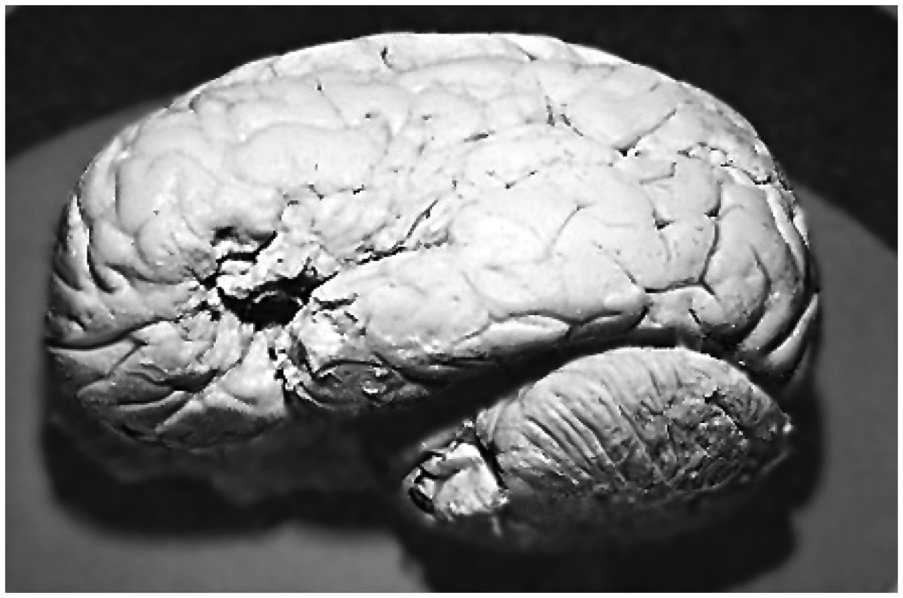
\includegraphics[width=6cm]{broca.png}
\end{center}
  \caption{\textbf{A picture of Broca's brain}; the lesion is clearly visible. Figure from
    \texttt{cambridge.org}\label{fig_broca}}
\end{figure}

These days, this neat division of the speech areas into Broca's area
and Wernicke's area, and aphasia into expressive and fluent aphasia,
is considered to binary; the function of these areas in language and
their ability to respond to insult is complex. Nonetheless it is
amazing to think that the linguistic ability, which we experience as a
unitary ability, can be subdivided into different abilities and these
abilities are localized in different areas. The neurologist Alexander
Luria even discovered that his patient Lev Alexandrovich Zasetsky who
received a severe brain injury in the second world war, had problems
with nouns to a far greater extent than he had problems with verbs.

\subsection*{The motor and somatosensory cortices}


\begin{figure}[tbhp]
  \begin{center}
  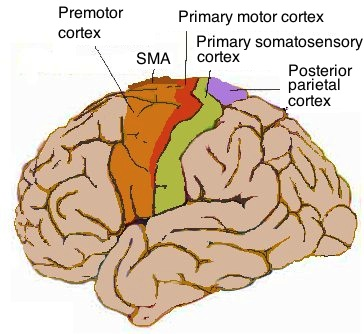
\includegraphics[width=6cm]{Human_motor_cortex.jpg}
\end{center}
  \caption{\textbf{The motor and somatosensory cortices}; the primary motor
    cortex is in red, the primary somatosensory cortex in green. Figure from
    \texttt{wikipedia}\label{fig_m_and_s}}
\end{figure}


Sticking to the cortex, in the first half of the C20 the neurosurgeon
Wilder Penfield pioneered a technique in neurosurgery, still important
today, of waking the patient up during the surgery and stimulating
parts of the brain: because the brain itself has no sensory nerve
endings this is painless, though it must be alarming. This allowed him
to work out which parts of the brain could be operated on, or removed,
while causing the least damage to crucial abilities. As a consequence
to this he discovered and mapped out the motor and somatosensory cortices,
Fig.~\ref{fig_m_and_s}. Touching parts of the motor cortex cause
movement in the patient, touching parts of the somatosensory cortex cause
fictive sensations. Different parts of each correspond to different
parts of the body, see Fig.~\ref{fig_motor} and the amount of space
dedicated to each part is proportional to how useful the information
is, rather than how big the part is, as illustrated in Fig.~\ref{fig_homunculus}.

\begin{figure}[tbhp]
  \begin{center}
  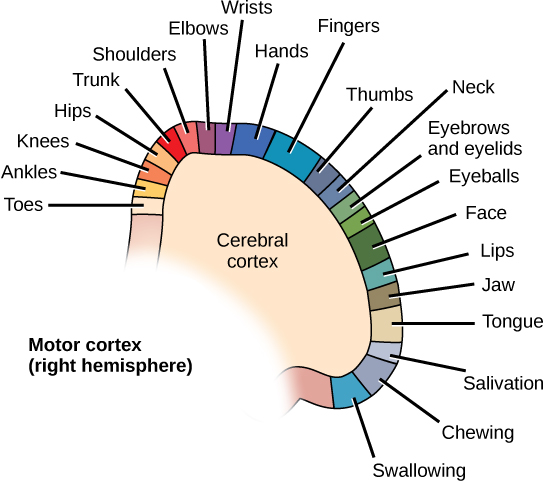
\includegraphics[width=6cm]{motor_mapping.jpg}
\end{center}
  \caption{\textbf{The motor cortex}; the map from cortex to parts of the body for the motor cortex, a similar map exists for the sensory cortex. Figure from
    \texttt{wikipedia}\label{fig_motor}}
\end{figure}


\begin{figure}[tbhp]
  \begin{center}
  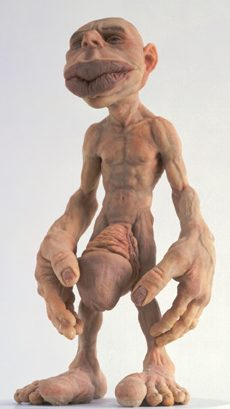
\includegraphics[height=5cm]{sensory.jpg}
\end{center}
  \caption{\textbf{The sensory homunculus}; this shows parts of the
    body proportional to how large an area is given over to it in the
    sensory cortex. I can't remember where I got this figure from and
    so I can't attest to its accuracy, you see other versions with
    smaller genitals, but that may be a bowlderisation, there is no
    corresponding female figure either, possibly for the same reason,
    or possibly because female neuroanatomy is less well studied, a
    problem common in neurology, neuroscience and psychology. This is
    discussed in this context in
    \cite{WrightFoerder2020}.\label{fig_motor}}
\end{figure}

This specialization of the sensory cortex is not restricted to the
somatosensory cortex, there are also parts of the cortex dedicated to
vision and hearing; the story with smell and taste is more
complicated. These are all primary sensory regions, they do initial
processing on the sensory information, but further processing, further
along the pathway, often includes the mixing of different pathways. It
is easy to see this happens by thinking how much easier it is to hear
what someone is saying if you can also see their lips, something we
have all become familiar with during the pandemic.

\subsection*{The cortex and memory}

The gradual realization that different parts of the cortex had
different functions lead scientists to assume that memory,
particularly long-term memory had a location in the cortex. This lead
to a series of studies by Karl Lashley who taught maze tasks to rats
and then lesioned parts of their cortex, see for example
\cite{Lashley1950}. He discovered that cortical lesions did affect rat
performance in the maze, but that there was no clear relationship
between where the lesion was and the consequence for memory, leading
him to suppose that memories were randomly deposited across the
cortex. We know now that accounts of cortical memory are not so
straight-forward, there are areas of the cortex linked to certain
types of memory and areas of the cortex more likely to store memories
than others, but it does indicate that there is no easy way to
describe the localisation of cortical function.

\subsection*{Summary}

The cortex is the outer layer of the brain, although it looks
homogenous at first glance different areas have different
functions. Based on a patient mostly known as Tan, Broca discovered an
area of the brain associated with speech, damage to this area causes
expressive aphasia. Conversely, damage to Wernicke's area caused
fluent aphasia, a lack of meaning rather than a lack of words. The
motor control and somatosensory perception of different parts of the
body is also linked to distinct brain areas, one for moving your left
pinkie, another for processing feelings from it, for example. In fact
there are cortical areas for primary processing related to hearing and
vision as well, but the localization of memory is less clearcut.

\bibliographystyle{plain}
\bibliography{../../misc/references}{}



\end{document}

